\let\negmedspace\undefined
\let\negthickspace\undefined
\documentclass[journal]{IEEEtran}
\usepackage[a5paper, margin=10mm, onecolumn]{geometry}
%\usepackage{lmodern} % Ensure lmodern is loaded for pdflatex
\usepackage{tfrupee} % Include tfrupee package

\setlength{\headheight}{1cm} % Set the height of the header box
\setlength{\headsep}{0mm}     % Set the distance between the header box and the top of the text

\usepackage{gvv-book}
\usepackage{gvv}
\usepackage{cite}
\usepackage{amsmath,amssymb,amsfonts,amsthm}
\usepackage{algorithmic}
\usepackage{graphicx}
\usepackage{textcomp}
\usepackage{xcolor}
\usepackage{txfonts}
\usepackage{listings}
\usepackage{enumitem}
\usepackage{mathtools}
\usepackage{gensymb}
\usepackage{comment}
\usepackage[breaklinks=true]{hyperref}
\usepackage{tkz-euclide} 
\usepackage{listings}
% \usepackage{gvv}                                        
\def\inputGnumericTable{}                                 
\usepackage[latin1]{inputenc}                                
\usepackage{color}                                            
\usepackage{array}                                            
\usepackage{longtable}                                       
\usepackage{calc}                                             
\usepackage{multirow}                                         
\usepackage{hhline}                                           
\usepackage{ifthen}                                           
\usepackage{lscape}
\begin{document}

\bibliographystyle{IEEEtran}

\title{12.765}
\author{EE25BTECH11023 - Venkata Sai}
% \maketitle
% \newpage
% \bigskip
\maketitle 
\renewcommand{\thefigure}{\theenumi}
\renewcommand{\thetable}{\theenumi}
\setlength{\intextsep}{10pt} % Space between text and floats

\numberwithin{align}{enumi}
\numberwithin{figure}{enumi}
\renewcommand{\thetable}{\theenumi}
\vspace{-1em}
\textbf{Question:}  \\
Let $\vec{v_1}=\myvec{1\\2\\0}$ and $\vec{v_2}=\myvec{2\\1\\3}$ be two vectors. The value of the coefficient $\alpha$ in the
expression $\vec{v_1} = \alpha \vec{v_2} +\vec{e}$, which minimizes the length of the error vector $\vec{e}$, is \\
\textbf{Solution:}  \\
Given expression
\begin{align}
    \vec{v_1} = \alpha \vec{v_2} +\vec{e}
\end{align}
where $\vec{e}$ is the error vector\\
 For any linear system $\vec{A}\vec{x}=\vec{B}$, the least squares solution formula is given by
 \begin{align}
     \brak{\vec{A}^\top\vec{A}}\vec{x}=\vec{A}^\top\vec{B} \\
     \vec{x}= \brak{\vec{A}^\top\vec{A}}^{-1}\vec{A}^\top\vec{B}
 \end{align}
 On writing the given expression as a linear system
 \begin{align}
     \vec{v_2}\alpha =\vec{v_1} 
 \end{align}
 where $\alpha$ being an 1$\times$1 vector
 \begin{align}
     \vec{A}=\vec{v_2},\vec{B}=\vec{v_1} 
     \end{align}
     \begin{align}
\alpha&=\brak{\vec{v_2}^\top\vec{v_2}}^{-1}\vec{v_2}^\top\vec{v_1} \\
    &= \brak{\myvec{2\\1\\3}^\top\myvec{2\\1\\3}}^{-1}\myvec{2\\1\\3}^\top\myvec{1\\2\\0} \\
     &= \brak{\myvec{2&1&3}\myvec{2\\1\\3}}^{-1}\myvec{2&1&3}\myvec{1\\2\\0} \\
     &=\brak{4+1+9}^{-1}\brak{2+2+0}\\
     &=\frac{1}{14}\brak{4}\\
     &=\frac{2}{7}
 \end{align}
 \begin{figure}[h!]
   \centering
   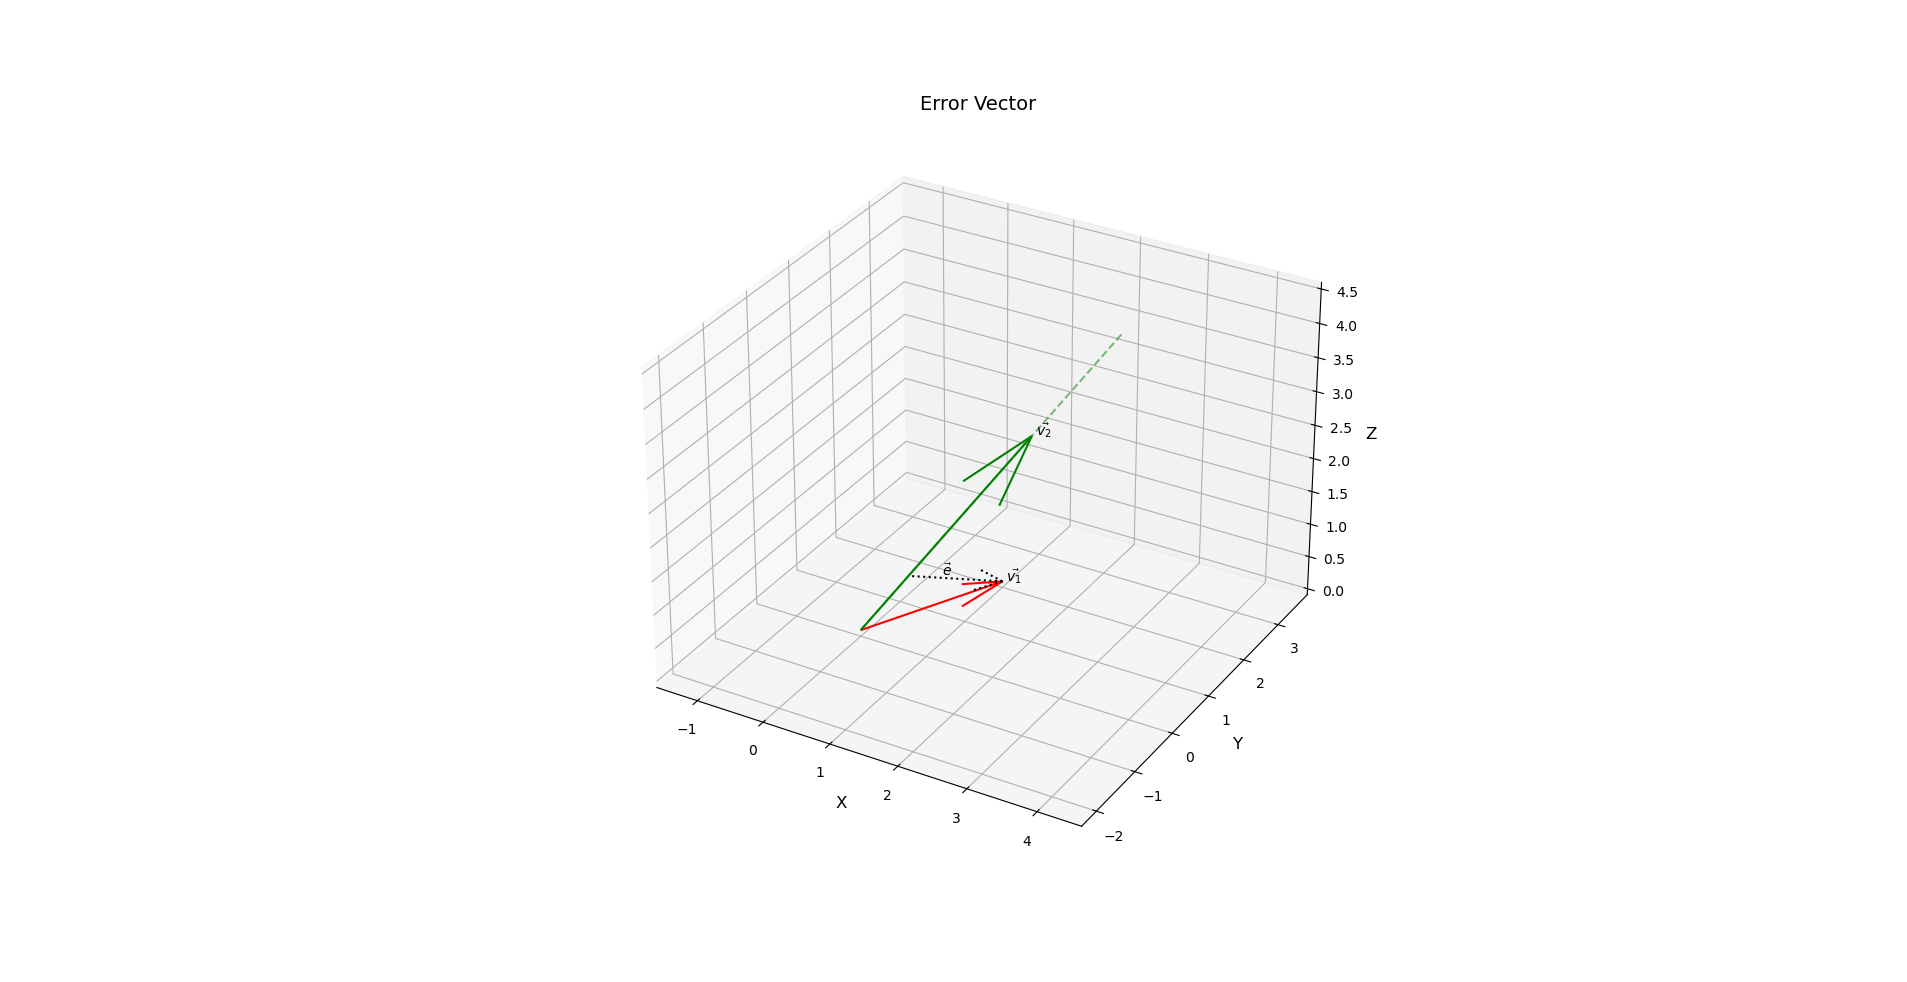
\includegraphics[width=1.\columnwidth]{figs/fig1.png}
	\caption{}
   \label{}
\end{figure}
 \end{document}
